\section{Introduction}
words
\subsection{What is Water Resources Management?}
Water resources management is:
\begin{quote}The activity of planning, developing, distributing and managing the optimum use of water
resources. Water resource management planning considers the competing demands for/
on water (quantity, quality, location, and timing) and seeks to allocate water on an
equitable basis to satisfy all uses and demands.
\end{quote}

Paraphrasing WRSPM:
\begin{quote}
The central purpose of water resources planning and management activities is to
address and, if possible, answer questions such as:\\
How can renewable yet finite water resources (e.g. rivers, estuaries, lakes, glaciers, and coastal zones) best be managed and used?
How can this management and use be accomplished in an environment of uncertain supplies and uncertain and increasing demands, and consequently of increasing conflicts among individuals having different interests in the management of a river and its basin?
\end{quote}

Key concepts/terms are
\begin{itemize}
\item Finite (limited) water resource.
\item How much, when, how yummy.
\item Allocate to many.
\item Equity/conflicts.
\item ``Best be managed $\dots$''
\end{itemize}
\newpage
\subsubsection{What is ``Allocate''}
Allocate means \\~\\
1: to apportion for a specific purpose or to particular persons or things : distribute
allocate tasks among human and automated components\\
2: to set apart or earmark : designate allocate a section of the building for special
research purposes\\

If the resource is abundant then allocation is unnecessary.  
However, water resources are identified as finite, hence limited in scope both spatially and temporally.

Because the resource is scarce; allocation will necessarily deny the resource to some, and supply it to others.

\subsubsection{What is ``Equitable''}
Equitable means \\~\\
1: having or exhibiting equity : dealing fairly and equally with all concerned an
equitable settlement of the dispute \\
2: existing or valid in equity as distinguished from law an equitable defense\\

Because the resource is scarce; allocation will necessarily deny the resource
to some, and supply it to others. 
Equity implies some kind of ?fairness? in that allocation.

\subsection{Decision Making}
The allocation requires decisions be made.
Decisions (policy) may involve the activity of an individual decision maker or collective decision maker(s).
These two classifications may make decisions quite differently, based on their roles, emotions, and goals.

\subsubsection{How do individuals and groups make decisions?}
Some people may seem indecisive or inconsistent. 
They may avoid making decisions as long as possible.
The same reluctance to make decisions also happens in organizations or institutions.
The decision avoidance may be an individual or collective desire to address uncertainty, in waiting, more information may become available.

On the other hand, some people and groups may be accused of ``jumping to conclusions" or making a decision ``without considering all the facts."
The decision acceleration may be an individual or collective assessment of the utility of more information, or a value judgement of the importance of the actual situation to longer term goals, or acknowledgement of urgency, or just plain laziness -- all of these explanations are clearly situational dependent.

This dichotomy itself contains a valuable implication that, in general, decisions should be made by collecting and weighing various elements in a rational way. 
Furthermore, alternatives must exist, or there is no decision to make.   

Decision making contains deep psychological aspects. People's choices depend upon how alternatives are
presented -- consider Figure \ref{fig:Picture1.png}.
\begin{figure}[h!] %  figure placement: here, top, bottom, or page
   \centering
   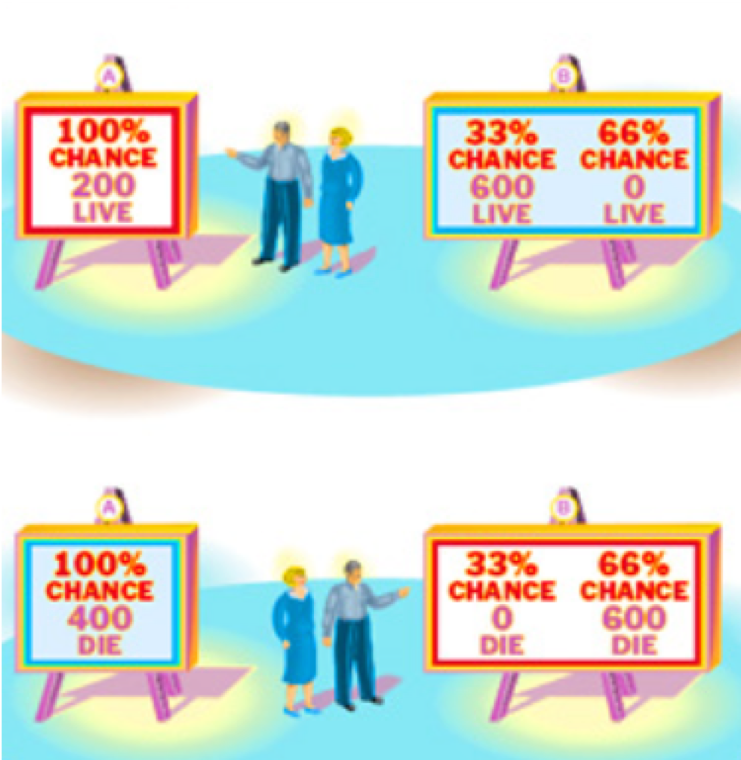
\includegraphics[width=6in]{./Lesson1/Picture1.png} 
   \caption{Identical decisions.  Upper panel is "Survival Based"; Lower panel is "Mortality Based" }
   \label{fig:Picture1.png}
\end{figure}
\newline
Consider the decision A or B,  the actual outcomes in terms of probability and number of survivors of the decision.\\
If we make decision A. The probability $P$ of the outcomes are $P(S=200) = \frac{1}{1}; P(S=0) = \frac{0}{1}$.
If we make decision B. The probability $P$ of the outcomes are  $P(S=600) = \frac{1}{3}; P(S=0) = \frac{2}{3}$.

Expectation in this structure is the product of the value of the outcome and the probability of that outcome.
Thus $E(S_A) = 1.0 \times 200 + 0.0 \times 0 = 200~\text{people}$, and  $E(S_B) = \frac{1}{3} \times 600 + \frac{2}{3} \times 0 =  200~\text{people}$.

Whichever decision is chosen A or B has the same expected outcome (in terms of expectation in the statistical sense); 200 people survive.
So one might conclude it does not matter which decision we make -- but that's not the whole story.  

While decision A guarantees 200 survive, decision B has a 66\% chance or zero survivors -- which is intended here to illustrate the influence of uncertainty in decision making.

Furthermore, how the situation is presented (Survival Based or Mortality Based) can have a severe emotional influence on how one would make the choice.

Lastly, consider the exogenous influences.  If the people in the example pay taxes, then the cost of the decision could influence the actual decision.

This simple example illustrates the challenges of something seemingly as simple as making a decision.

\subsection{Challenge of Water Resources Management}
There are actually only a few challenges (at a very high cognitive level):
\begin{itemize}
\item Define alternatives (present decision points)
\item Define value
\item Define outcomes
\item Define equity; ``what is fair'' for a situation
\item Implement tools to support (defend) the decision
\item Implement the decision(s)
\end{itemize}

\subsubsection{Support Tools}
One of the bullet items is tools to support the decision.  
These include economics or some other way to value the alternatives (cost and benefit), as well as measure ``fairness''
Then some policy (or procedure) to rank the value(s).
Another policy or procedure to guide the decision -- in some instances we could hand off the decision to an algorithm (Narrow Domain AI).  We already let such algorithms fly aircraft with us in them, recommend products for us to purchase, detect fraudulent fiscal activity and such.
Another important factor in the support/implementation component is what level of control do we have.
\begin{itemize}
\item Do we control the system? \\
SCADA operating a water distribution network -- fully autonomous with little human intervention.
%Autopilot algorithm to operate a commercial aircraft -- fully autonomous with little human intervention.
\item $\dots$ or just influence the system \\
Voluntary compliance versus risk of apprehension for water quality management
\end{itemize}

%\subsubsection{Example}
%\subsection{Assigning Value}
%\subsubsection{Example}
%\subsection{Readings}
%\subsection{Exercises}